Once more, we took advantage of the application insight capabilities to store and aggregate logs coming from the backend service, with a maximum retention policy of 30 days. To achieve that we have intercepted each request coming toward our controller request handler using aspect-oriented programming to register the request in a logging agent, namely Logback which we have registered in application insight, and explicitly tracing the event triggered from the controller method handler to the business level, data access level and back again. We have set up the logging level to be configured at run time using spring profiler and changing the log. Level attribute to be: info, trace, debug if needed. As a result, we have a control panel in Azure that shows our logging and aggregation, including response time and failed requests aggregation function. Moreover, the trace provided by logback.spring integration gave us the ability to drill down into the logs and trace the route and messages after execution.
\begin{figure}
    \centering
    \begin{subfigure}[b]{0.45\textwidth}
        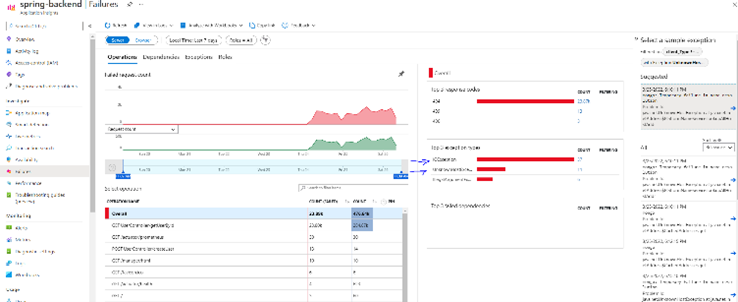
\includegraphics[width = \textwidth]{springbackendinfo.png}
    \end{subfigure}
    \hfill
    \begin{subfigure}[b]{0.45\textwidth}
        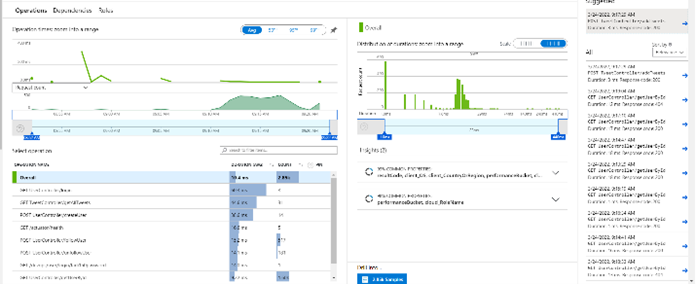
\includegraphics[width = \textwidth]{idunno.png}
    \end{subfigure}
    \caption{Log revelation}
    \label{fig:screenshots}
\end{figure}
The logs reveal an important issue to the developers which was a known bug in spring container dependency injection context when running on our Linux distribution version. Fortunately, the error did not cause the service to crash, and it occurred only while the cron-job in Linux was running, so we let it be since it seemed to be harmless.
